\title{Final Project Description}
\documentclass[11pt]{article}

%%
%% packages
%%

\usepackage[T1]{fontenc}
\usepackage[utf8]{inputenc}
%\usepackage[icelandic]{babel}
\usepackage{amsfonts}
\usepackage{amssymb}
\usepackage{amsmath}
\usepackage{courier}
\usepackage{amsthm} % for theoremsyles
\usepackage{float}
\usepackage{geometry}
\usepackage{graphicx}
\usepackage{color, colortbl}
\usepackage{pdflscape}
\usepackage{pbox}
\usepackage{tabularx}
\usepackage{makecell}
\usepackage{verbatim}
\usepackage{enumerate}
\usepackage{listings}
\usepackage{hyperref}
\usepackage{tikz}
\usepackage{tikz-qtree}
\usepackage{verbatimbox}
\usepackage{url}
\definecolor{LightSteelBlue}{rgb}{0.69,0.77,0.9}
\definecolor{Mint}{RGB}{198,230,162}
\definecolor{mygray}{gray}{0.6}
\definecolor{javared}{rgb}{0.6,0,0} % for strings
\definecolor{javagreen}{rgb}{0.25,0.5,0.35} % comments
\definecolor{javapurple}{rgb}{0.5,0,0.35} % keywords
\definecolor{javadocblue}{rgb}{0.25,0.35,0.75} % javadoc
 
\lstset{language=Java,
basicstyle=\ttfamily,
keywordstyle=\color{javapurple}\bfseries,
stringstyle=\color{javared},
commentstyle=\color{javagreen},
morecomment=[s][\color{javadocblue}]{/**}{*/},
numbers=left,
numberstyle=\tiny\color{black},
stepnumber=2,
numbersep=10pt,
tabsize=4,
showspaces=false,
showstringspaces=false}

%%
%% setup
%%

\geometry{a4paper, bottom = 4cm}


\makeatletter
\renewcommand\paragraph{\@startsection{paragraph}{4}{\z@}%
            {-2.5ex\@plus -1ex \@minus -.25ex}%
            {1.25ex \@plus .25ex}%
            {\normalfont\normalsize\bfseries}}
\makeatother
\setcounter{secnumdepth}{4} % how many sectioning levels to assign numbers to
\setcounter{tocdepth}{4}    % how many sectioning levels to show in ToC
%%
%% beginning of document
%%

\begin{document}
 \newcommand{\HRule}{\rule{\linewidth}{0.5mm}}
\begin{titlepage}

\begin{center}
% Upper part of the page

\includegraphics[width=0.55\textwidth]{./rulogo}\\[4.0cm]    

%\textsc{\LARGE Háskólinn í Reykjavík}\\[1.5cm]

\textsc{\LARGE Final Project}\\[0.5cm]
%\textsc{\Large Dæmatímaverkefni 8}\\[0.6cm]

% Title
\HRule \\[0.4cm]
{ \Huge \bfseries Work Schedule and Procedures}\\[0.4cm]

\HRule \\[1.5cm]


% Author and supervisor
\begin{minipage}{0.49\textwidth}
\begin{flushleft} \large
\emph{Students:}\\
Hjalti Leifsson \\
Jóhann Örn Bjarkason
\end{flushleft}
\end{minipage}
\begin{minipage}{0.49\textwidth}
\begin{flushright} \large
\emph{Teachers:} \\
Hallgrímur Arnalds \\
Hannes Pétursson \\
Hlynur Sigurþórsson
\end{flushright}
\end{minipage}

\vfill

% Bottom of the page
{\large \today}



\end{center}

\end{titlepage}
\date{\today}
\clearpage

\section{Introduction}\label{sec:introduction}

In this report we discuss the progress of our final project, \emph{Project Discovery}. In section~\ref{sec:time} we list the hours we have spent so far on the project in total and for each of us. In section~\ref{sec:burndown} we show the status of the burndown chart at this point, after four sprints have been completed. In section~\ref{sec:backlog} we go over the sprint backlogs of the sprints we've done so far and show the burndown charts for each sprint we have completed. Lastly in section~\ref{sec:retrospectives} we summarize our sprint planning and retrospective meetings. 

\section*{Background}
\section*{Description}
As stated above, this project started in January 2015 and the first few months of the project served as the final project at Reykjavík University by Gunnar Þór Stefánsson and Þór Adam Rúnarsson. They continued their work with a grant from Rannís. Gunnar had to leave the project in the beginning of July and Hjalti replaced him so Hjalti was already well up to speed when this semester started. 
 
To explain our part in the project we first go over what has been done already and the bigger picture of the project. The project is a so called Citizen Science project. Citizen Science (also known as crowd-sourced science) is scientific research conducted by many amateur or non-professional scientists. A lot of research must be performed by humans since no computational alternative exists and Citizen Science can help speed up research of that kind. 

MMOS (Massively Multiplayer Online Science), which is one of the companies behind the project, is trying to find new ways to conduct Citizen Science by mobilizing players in online video games to take part in the research. The idea is to make the research a seamless part of the gameplay and offer in-game rewards to encourage players to take part. This project, which is called \emph{Project Discovery} within \emph{EVE Online}, focuses on creating a game with a purpose in the \emph{EVE Universe} which will serve as a platform for research tasks. In this incarnation \emph{Project Discovery} will involve players in identifying protein patterns in images of cells and then classifying them in the correct category. This is done in conjunction with \href{http://www.proteinatlas.org/subcellular}{The Human Protein Atlas} which provides the images to be analyzed. In the future Project Discovery could be used for other similar research tasks within the EVE universe.

\section*{Current status of the project}

When we took over the project in the beginning of the semester a lot of the work on the mini-game had already been done.
The game has an API from MMOS it can talk to in order to receive images for players, and score them based on their performance (in-game it is called "Accuracy Rating"). Players can therefore receive tasks and make selections on that task, based on available categories. They can then submit the task, and get-in game rewards and an updated accuracy score. Players receive a message, thanking them for their contribution, after each submitted task. They also receive in-game experience. Players level up with experience and can figuratively reach an endless level, there is no set limit. The highest level, for which you receive rewards for achieving, is level 100. Players also receive milestone titles for reaching certain level thresholds, such as: "Novice Analyst".

\begin{figure}[H]
	\centering
    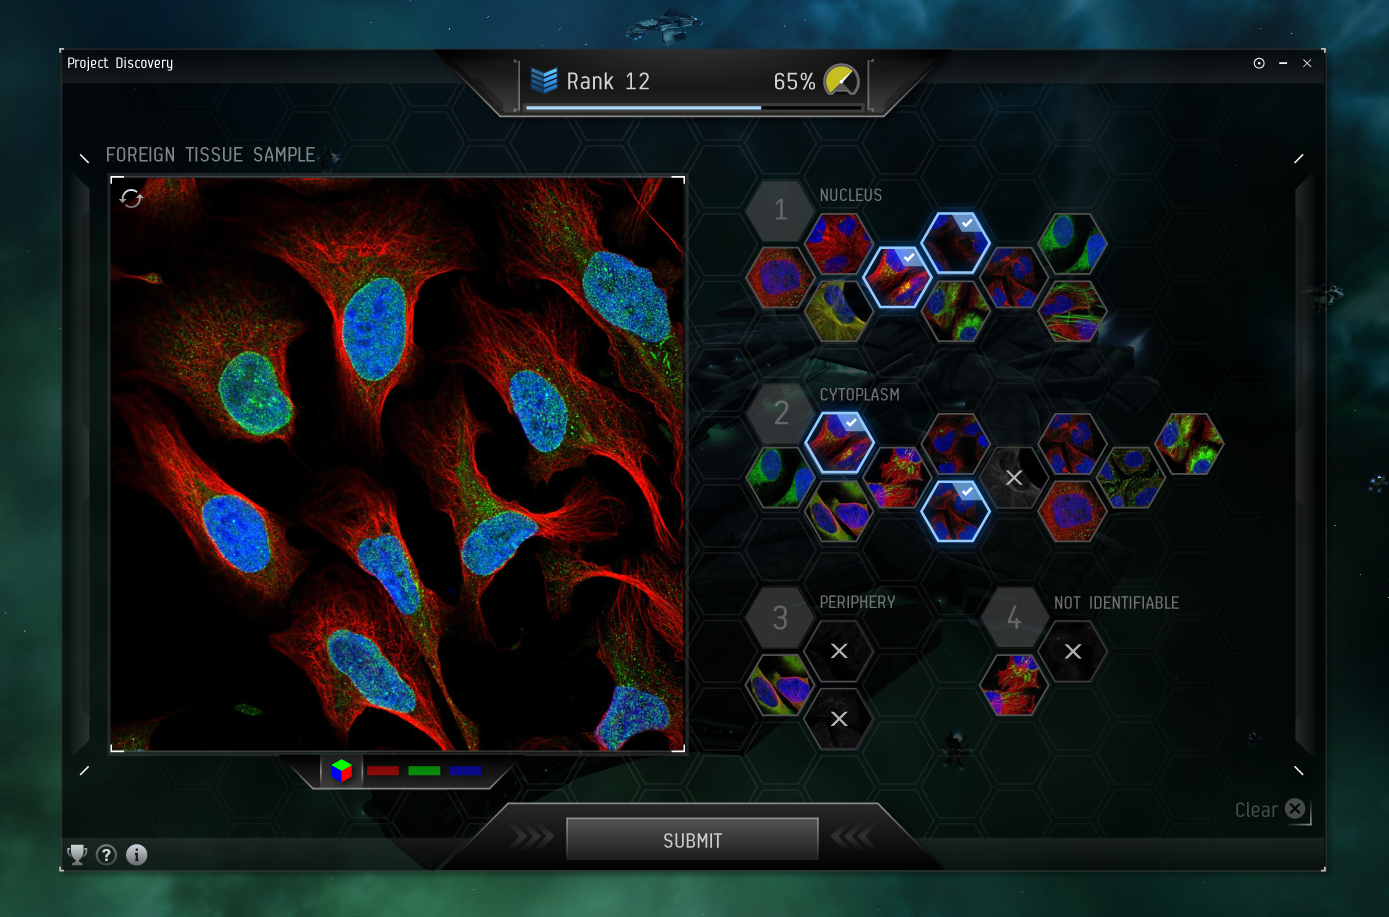
\includegraphics[width=15cm]{PD.png}
    \caption{\label{fig:PD}This is the design of the UI at this point}
\end{figure}

\section*{Outcome of the project}

Two main outcomes are expected by the end of the project. One is to implement the remaining features of \emph{Project Discovery}, and launch it on the \emph{EVE Online} test server, \emph{Singularity}. The other is to develop and launch a website dedicated to \emph{Project Discovery} that details its progress and player statistics, as well as informs the players and general public about it.\\

These are the main remaining features that we expect to be able to finish for this project:
\begin{itemize}
  \item A training phase where players get easy tasks and a few categories to solve.
  \item A detailed rewarding system, where players complete daily challenges for further rewards.
  \item A leaderboard, where players compete to be the best of the best.
  \item A detailed view of the history of player submissions, where each player can see what submission changed their score.
\end{itemize}

We also need to clear up a few things regarding authorization, optimization, player statistics tracking and how our client will be able to connect to the external MMOS API.\\

After release on the test server (or before, it is undecided), our task is to develop a website to launch along with the mini-game. At this point no development or design has been done on the website and only very basic discussion has taken place on the content of it, so the web development part of the project is likely to change and expand in scope. What we know currently is that it will contain information about \emph{Project Discovery} and it will in some way show the progress the \emph{EVE} players are making with the research, for an example how many pictures have been analyzed and how many more need to be analyzed.

\section*{About the companies (from the project proposal)}
CCP is a leading independent developer of massively multiplayer games, and has
been praised for its artistry, game design and unique player-driven, infinitely scalable
storytelling narratives. In addition to \emph{EVE Online}, CCP also develops \emph{DUST 514\textsuperscript{\textregistered}}, a
groundbreaking, free-to-play, massively multiplayer online first-person shooter for
the PlayStation\textsuperscript{\textregistered}3, and \emph{EVE: Valkyrie™}, a multiplayer spaceship dogfighting shooter, both set in the EVE Universe. Founded and headquartered in Reykjavik,
Iceland, in 1997, CCP is privately held, with additional offices in Atlanta, Newcastle,
and Shanghai. For more information, visit \href{http://www.ccpgames.com/}{ccpgames.com}.\\

MMOS is a privately held start-up company from Switzerland specializing in the field
of citizen science. The company was founded in 2014 by Attila Szantner and
Bernard Revaz. Mr. Szantner has a long history in the field of IT, amongst other
projects being one of the creators of iwiw.hu (the Hungarian “Facebook” which at its
height \href{http://en.wikipedia.org/wiki/IWiW}{reached more than 4 million users}). Mr.
Revaz has 15 years of research history in physics (University of Geneva, University
of California, EPLF).\\


CADIA is a highly innovative interdisciplinary centre at Reykjavík University that
explores and extends the relationship between humans and intelligent machines
through deep understanding and modeling of human behaviour, design of real-time
sensing and decision making mechanisms, and extensive prototyping and evaluation
methodology. CADIA’s projects have received numerous international awards and
honours, including being three times winners of the international General Game
Playing (GGP) competition, two times recipients of the Kurzweil Award for Artificial
General Intelligence (AGI) and placing fourth at the international Autonomous
Underwater Vehicle (RoboSub) competition. CADIA contains 8 faculty members and
over 40 research staff and students. Learn more at \href{http://cadia.ru.is/}{cadia.ru.is}.
\end{document}
